\chapter{Requirements}
\label{ch:requirements}
\section{Requirements Elicitation}

\subsection{Persona}
Kevis represents trend-oriented users who actively seek style inspiration and enjoy experimenting with new outfits. This persona is important because it reflects a core user group that benefits most from personalized recommendations and virtual try-on features. It directly supports the system requirements for personalized recommendations and outfit generation.

\begin{figure}[H]
    \centering
    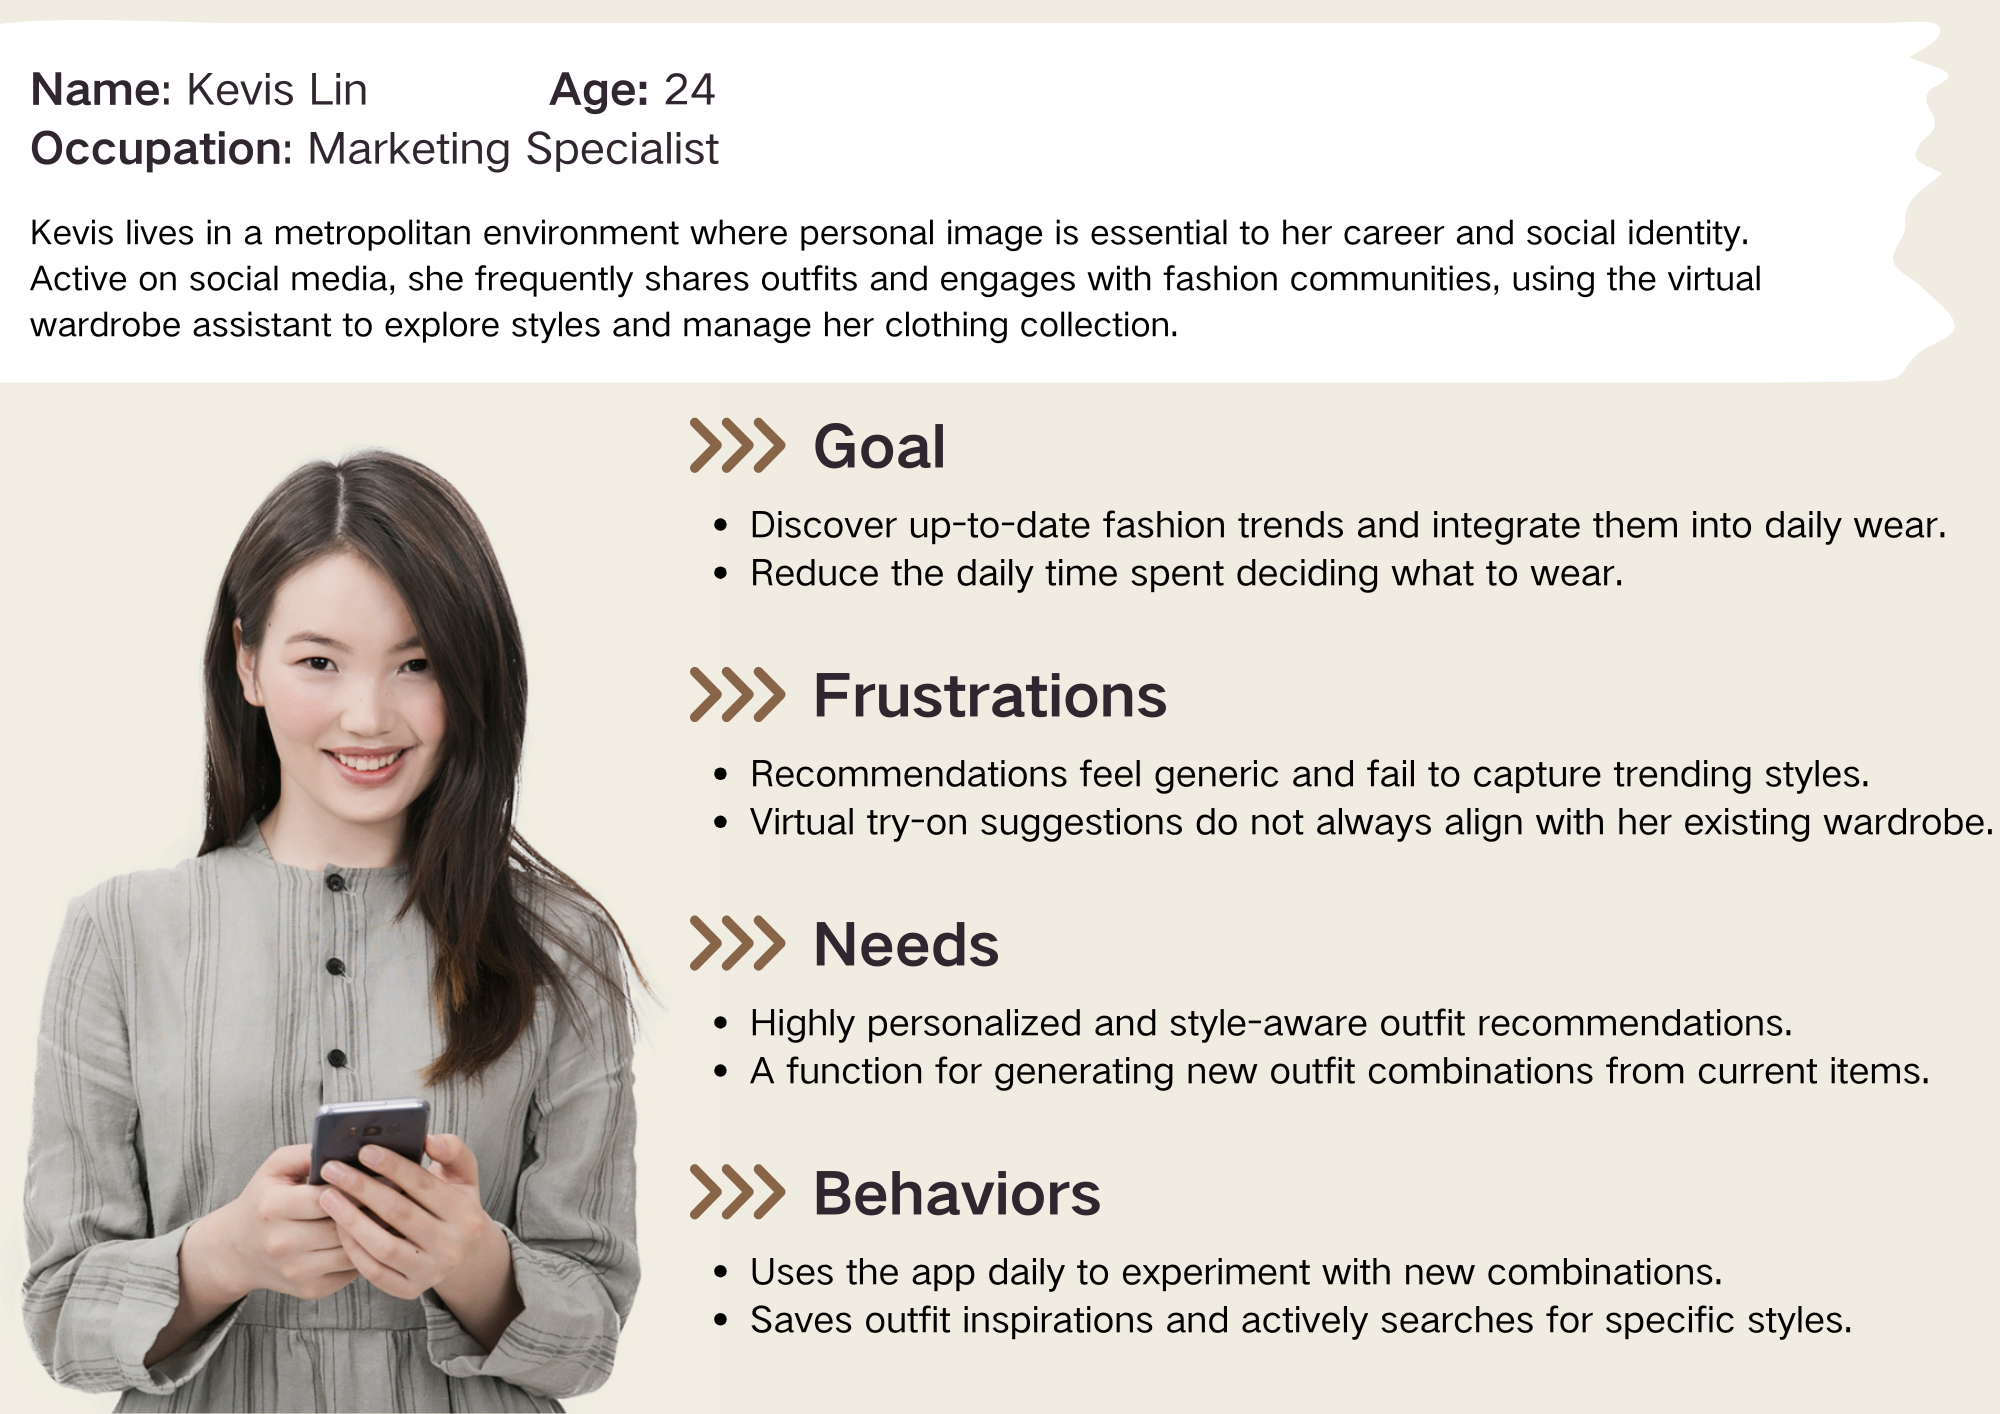
\includegraphics[width=0.80\textwidth]{images/Section_4_requirement/persona1.png}
    \caption{Fashion Explorer's persona}
    \label{fig:Kevis}
\end{figure}

Joe represents efficiency-focused users who want quick, reliable outfit decisions for professional settings. This persona is important because it highlights the need for weather-aware, occasion-appropriate recommendations and clear wardrobe organization. It directly supports the system requirements for weather-integrated recommendations and efficient wardrobe organization.

\begin{figure}[H]
    \centering
    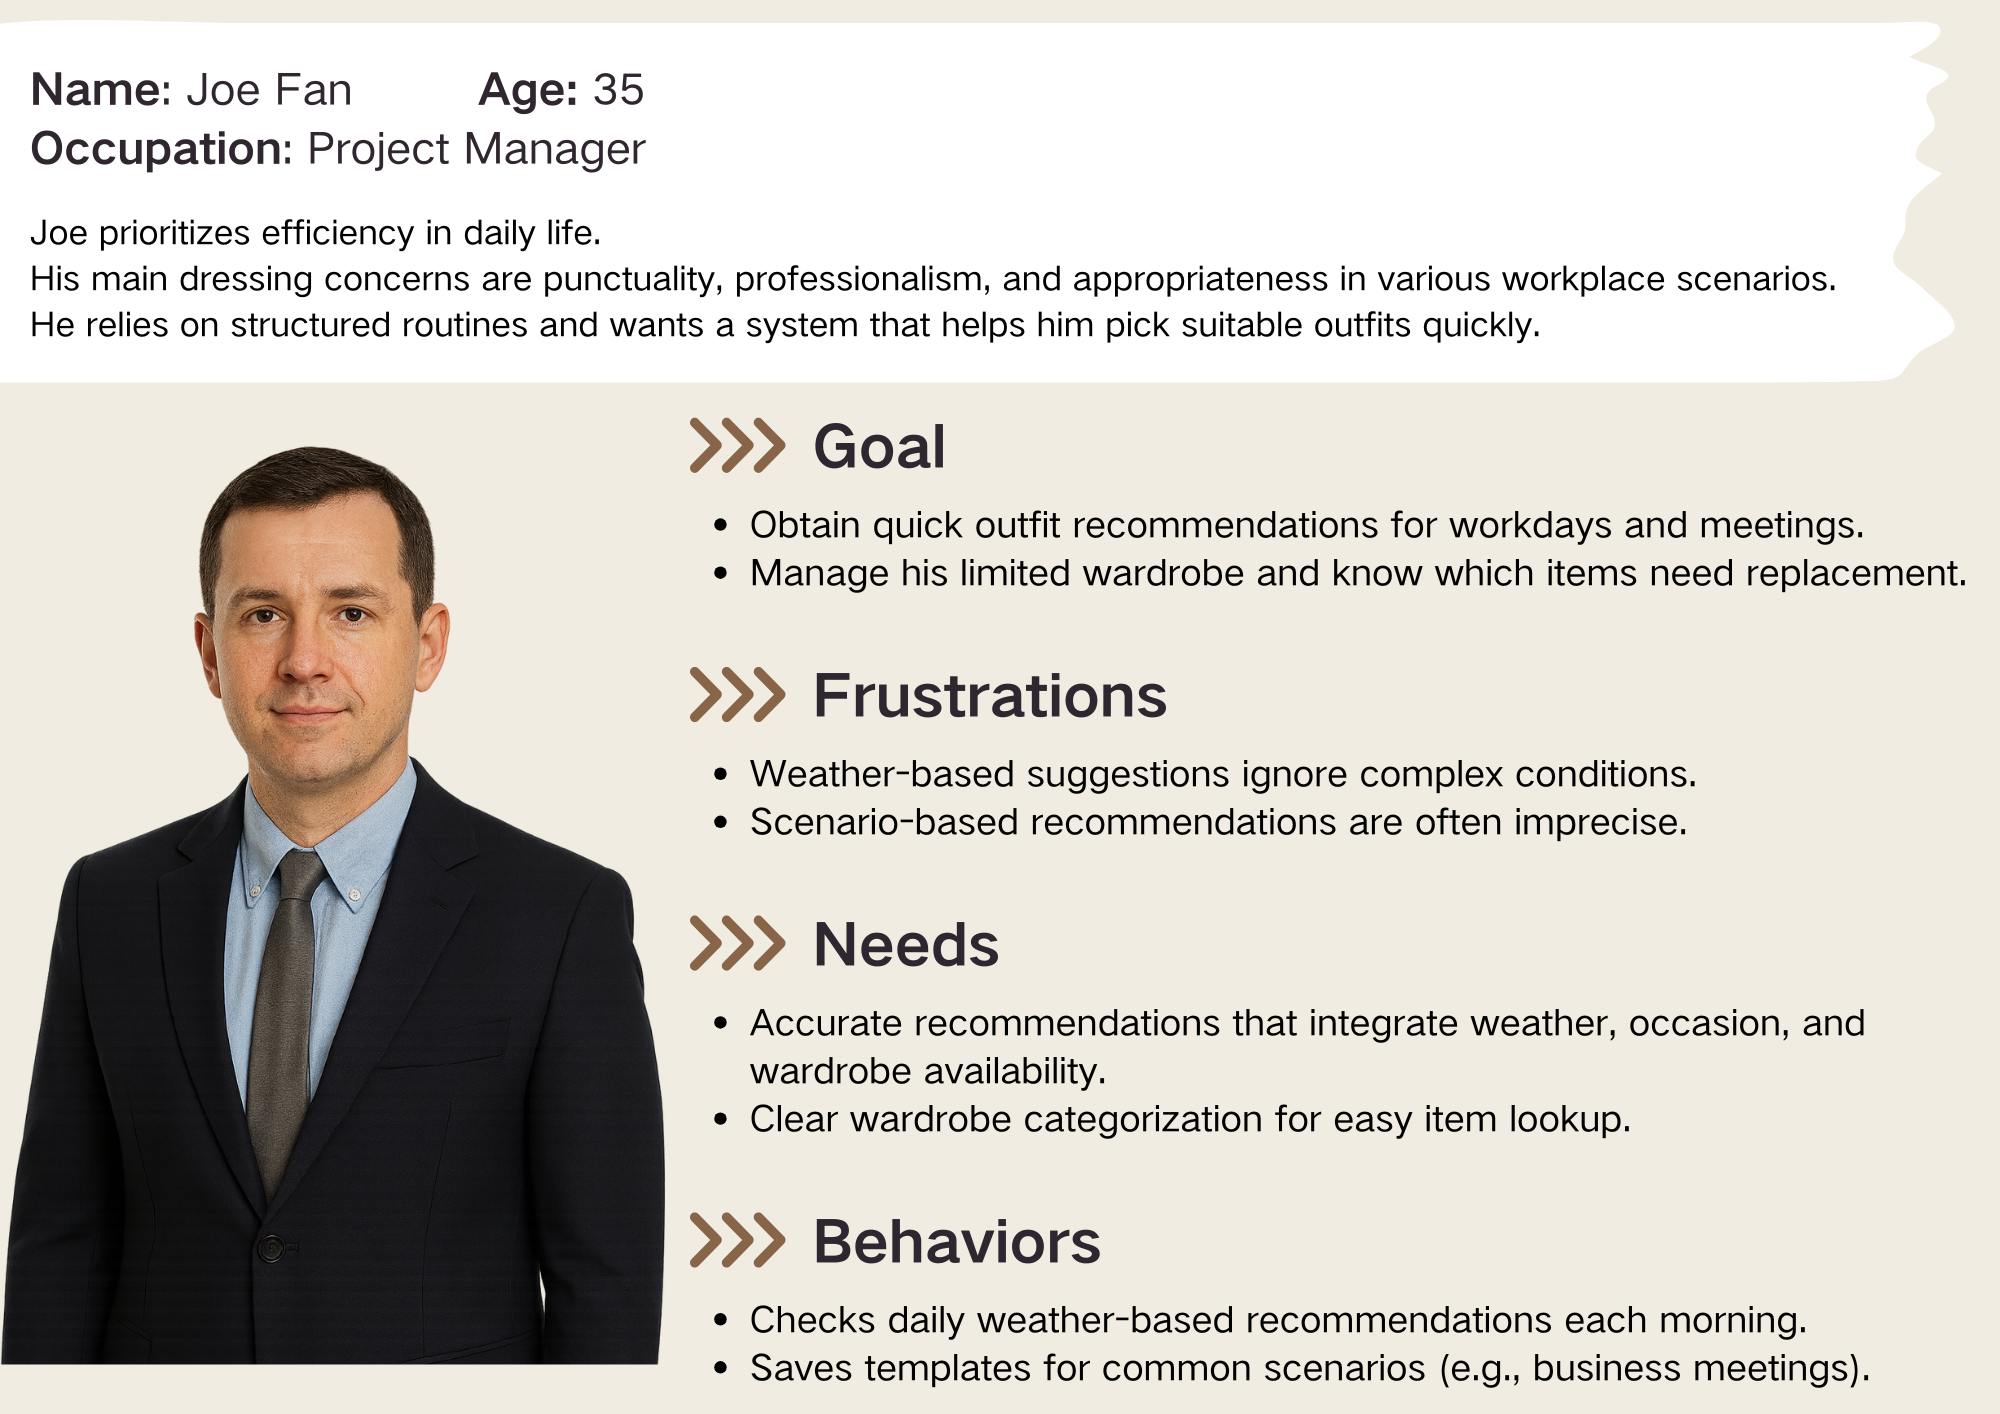
\includegraphics[width=0.80\textwidth]{images/Section_4_requirement/persona4.png}
    \caption{the Practicalist's persona}
    \label{fig:Joe}
\end{figure}

Jonathan represents the system-side stakeholder responsible for ensuring platform stability and user retention. This persona is important because his needs underscore the reliance on a scalable recommendation architecture and reliable performance. It directly supports key system requirements for model updates, data management, and continuous optimization.

\begin{figure}[H]
    \centering
    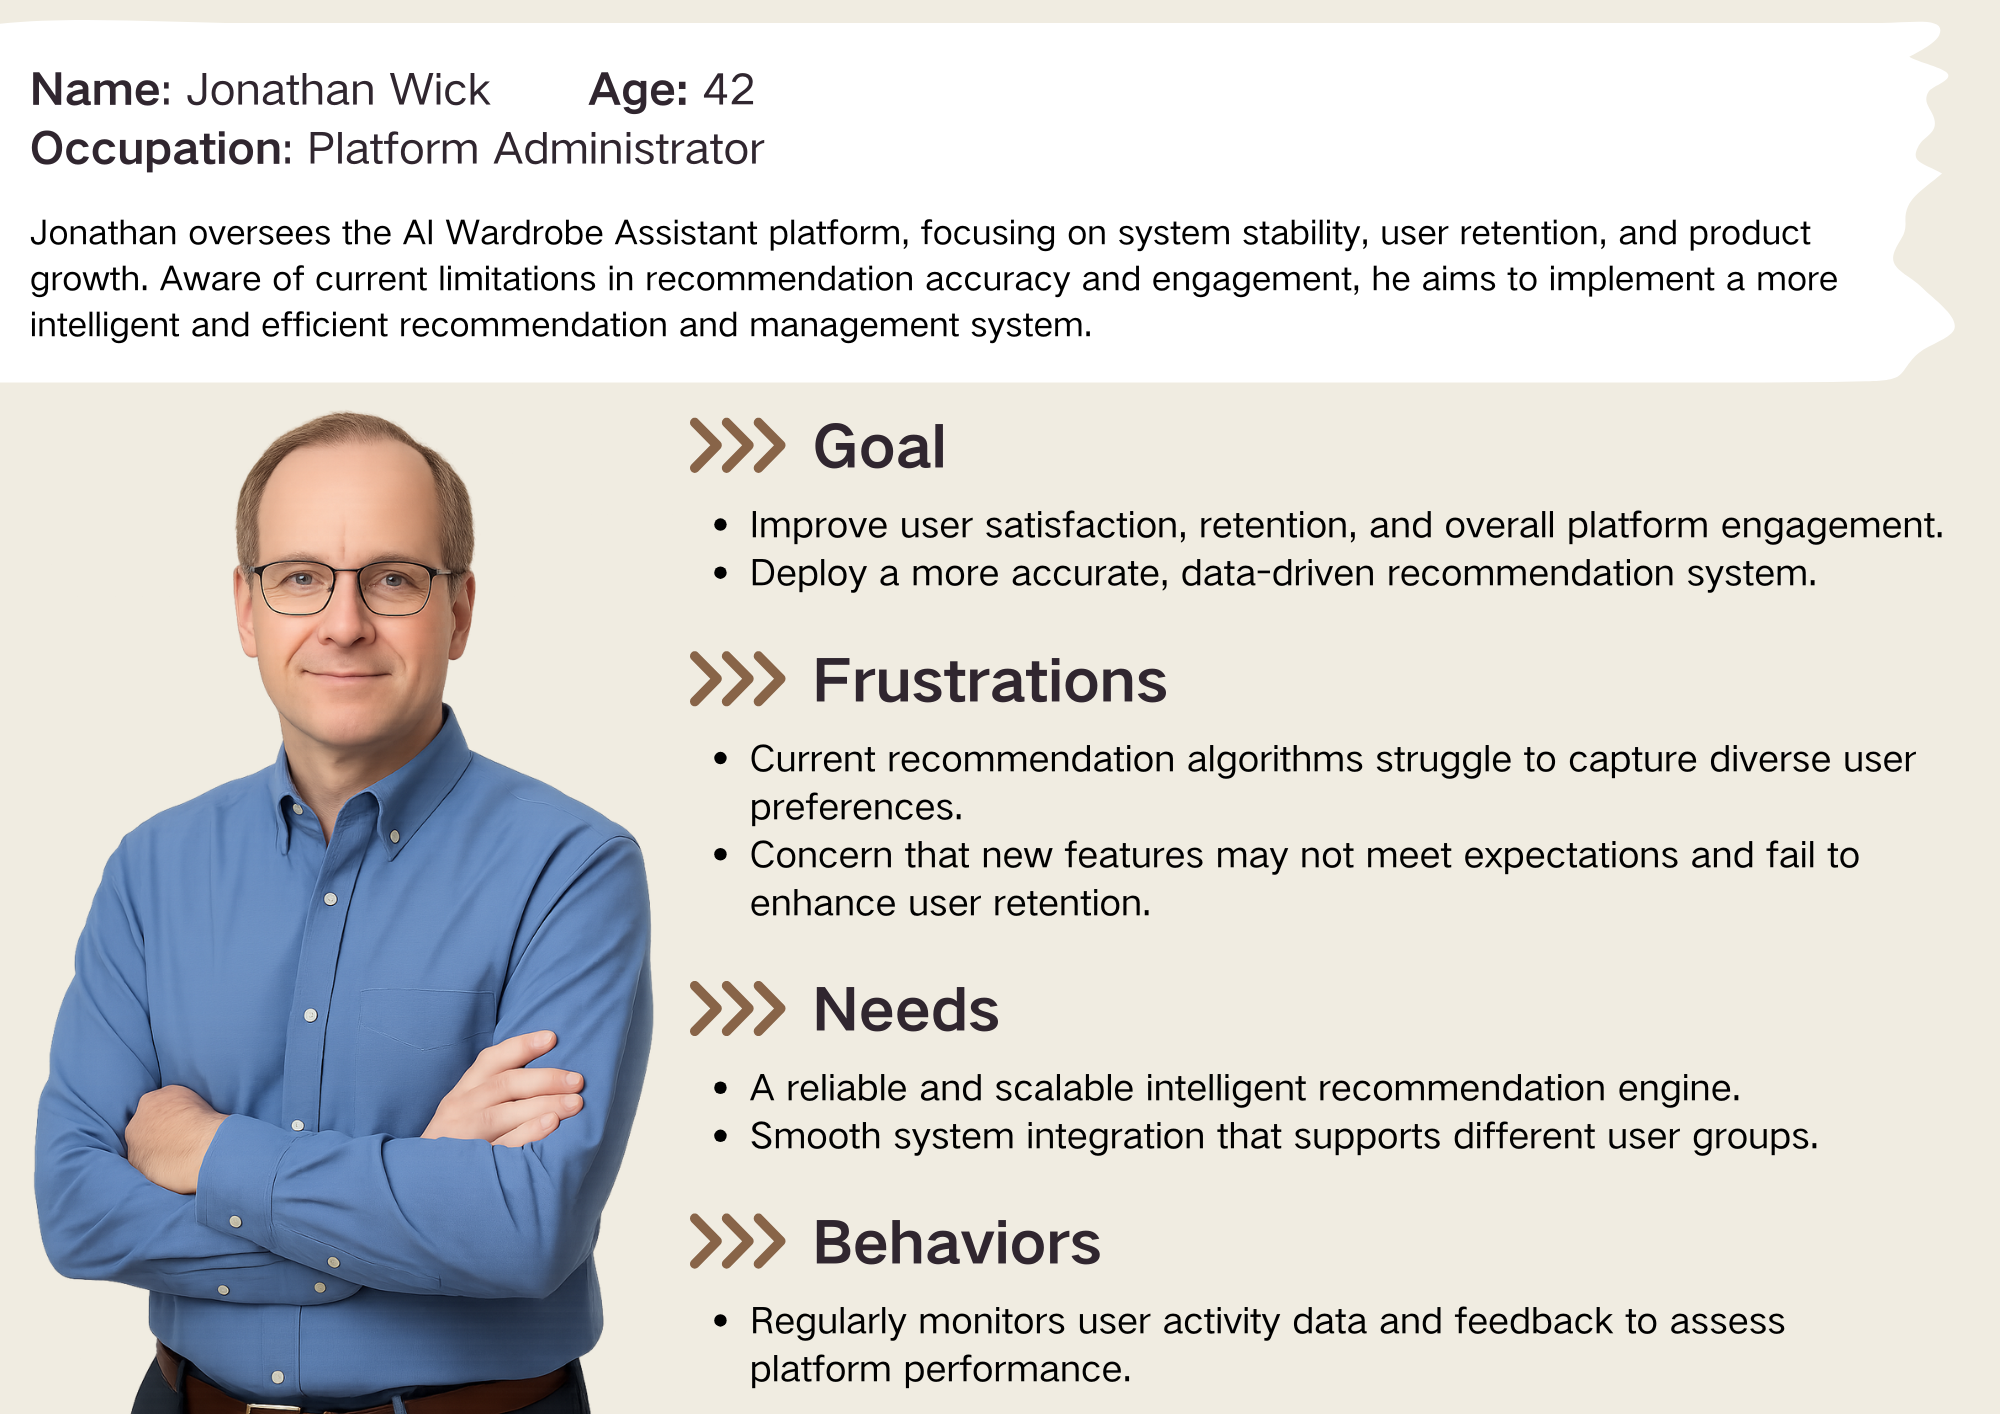
\includegraphics[width=0.80\textwidth]{images/Section_4_requirement/persona2.png}
    \caption{System Administrator's persona}
    \label{fig:Jonathan}
\end{figure}

Kiki represents users who prioritize practicality and reducing clothing waste. This persona is important because it highlights the need for style-compatible recommendations grounded in existing wardrobe items, as well as insights into usage patterns. It directly supports system requirements related to wardrobe analysis, outfit generation, and virtual try-on.

\begin{figure}[H]
    \centering
    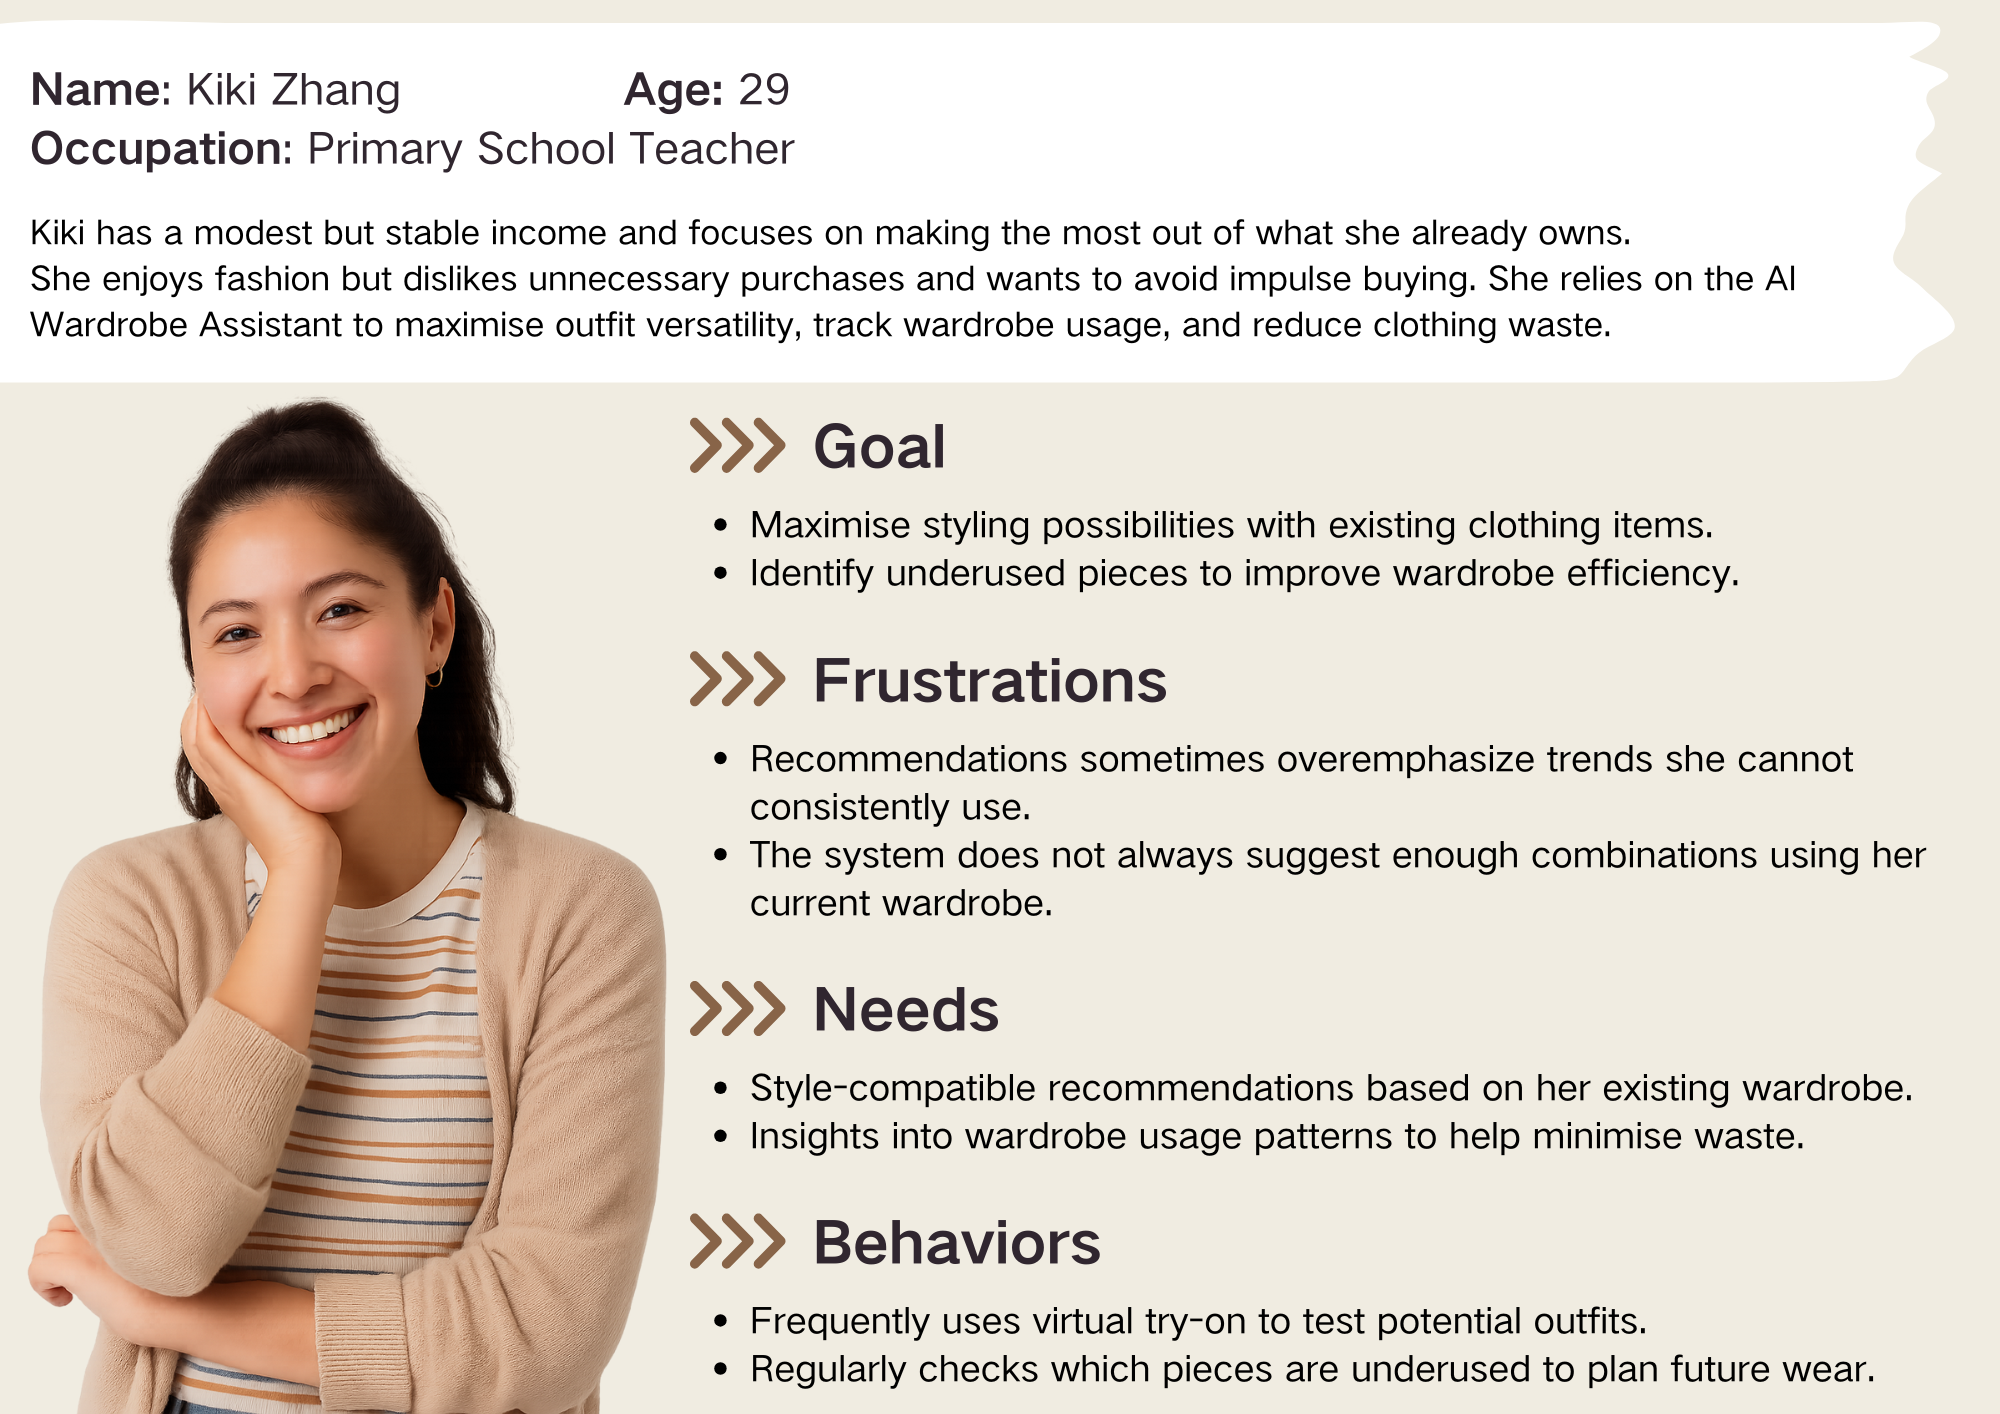
\includegraphics[width=0.80\textwidth]{images/Section_4_requirement/persona3.png}
    \caption{Wardrobe Optimizer's persona}
    \label{fig:Kiki}
\end{figure}


\subsection{User Story}

\textbf{\large 1. Kevis Lin — Fashion Explorer}\\

\textbf{US1.}\\
As a fashion enthusiast, I want personalized and trend-aware outfit recommendations so that I can remain stylish and express my unique identity.

\textbf{US2.}\\
As someone who frequently experiments with outfits, I want quick and relevant style suggestions so that I can reduce the time spent deciding what to wear each day.\\

\textbf{\large 2. Joe Fan — The Practicalist}\\

\textbf{US3.}\\
As a busy professional, I want one-click outfit suggestions based on weather and occasion so that I can dress appropriately with minimal effort.

\textbf{US4.}\\
As a wardrobe manager, I want my clothes clearly categorized in the app so that I can quickly find items.\\

\textbf{\large 3. Jonathan Wick — System Administrator}\\

\textbf{US5.}\\
As a data-driven operator, I want to analyze user behavior so that I can optimize future improvements.\\

\textbf{\large 4. Kiki Zhang — Wardrobe Optimizer}\\

\textbf{US6.}\\
As a wardrobe optimizer, I want guidance on styling items I already own so that I can maximize the value of my wardrobe.

\section{Requirement Specification}
\subsection{Functional Requirements}
\begin{table*}[ht]
\centering
\small
\caption{Functional Requirements (FR)}
\label{tab:functional_requirements}
\begin{tabular}{p{1.6cm}p{13.2cm}}
    \toprule
    \textbf{FR ID} & \textbf{Description} \\
    \midrule
    FR-01 &
    The system must support user registration, login, logout, and initialize wardrobe setup after first login. \\
    
    FR-02 &
    The system must allow users to add clothing items via structured forms (basic attributes, metadata, photos). \\
    
    FR-03 &
    The system must support batch image uploads and automatically generate candidate tags based on visual attributes. \\
    
    FR-04 &
    The system must maintain a user preference profile and allow users to edit personal preferences. \\
    
    FR-05 &
    The system must allow users to input outfit constraints, including occasion, etiquette, comfort level and color choices. \\
    
    FR-06 &
    The system must automatically retrieve weather conditions based on user location and date, with an option for manual override. \\
    
    FR-07 &
    The system must generate no fewer than three outfit recommendations that satisfy occasion, weather and preference constraints. \\
    
    FR-08 &
    The system must provide explanation for each recommendation and offer alternative items or outfits for adjustment. \\
    
    FR-09 &
    The system must collect user feedback (like/dislike/avoid) and update preference learning for future recommendations. \\
    
    FR-10 &
    The system must allow users to upload full-body photos and preview outfit try-on results on their own images. \\
    
    FR-11 &
    The system must support try-on using clothing photos by segmenting and aligning garments for preview. \\
    
    FR-12 &
    The system must support exporting or sharing try-on results in image format or via shareable links. \\
    
    FR-13 &
    The system must support wardrobe maintenance, including search, filtering, batch editing and deletion. \\
    \bottomrule
\end{tabular}
\end{table*}


\newpage
\subsection{Non-Functional Requirements}
\subsubsection{Performance Requirements}

\begin{table}[H]
\centering
\small
\caption{Performance requirements (NFR)}
\label{tab:nfr_performance}
\begin{tabular}{p{1.2cm}p{13.2cm}}
\toprule
\textbf{NF ID} & \textbf{Description} \\
\midrule
NF-01 & The system should respond to user recommendation requests within 3 seconds. \\
NF-02 & The system should support concurrent users without significant performance degradation. \\
NF-03 & The virtual try-on rendering for a single 720p image should be completed within 10 seconds. \\
\bottomrule
\end{tabular}
\end{table}


\subsubsection{Usability Requirements}

\begin{table}[H]
\centering
\small
\caption{Usability requirements (NFR)}
\label{tab:nfr_usability}
\begin{tabular}{p{1.6cm}p{13.2cm}}
\toprule
\textbf{NF ID} & \textbf{Description} \\
\midrule
NF-04 & The UI should follow a clean and consistent visual style. \\
NF-05 & Key functions (upload, recommendation, sharing) should require no more than three clicks or steps. \\
NF-06 & New users should be able to complete registration and wardrobe setup within 2 minutes. \\
NF-07 & The system should provide English and Chinese language switching. \\
\bottomrule
\end{tabular}
\end{table}


\subsubsection{Security and Privacy Requirements}

\begin{table}[H]
\centering
\small
\caption{Security and privacy requirements (NFR)}
\label{tab:nfr_security}
\begin{tabular}{p{1.6cm}p{13.2cm}}
\toprule
\textbf{NF ID} & \textbf{Description} \\
\midrule
NF-08 & User-uploaded personal photos should be used exclusively for the virtual try-on function and not for any other purpose. \\
NF-09 & The system should allow users to delete their accounts and personal data at any time. \\
\bottomrule
\end{tabular}
\end{table}


\subsubsection{Reliability Requirements}

\begin{table}[H]
\centering
\small
\caption{Reliability requirements (NFR)}
\label{tab:nfr_reliability}
\begin{tabular}{p{1.6cm}p{13.2cm}}
\toprule
\textbf{NF ID} & \textbf{Description} \\
\midrule
NF-10 & The system shall maintain an annual availability of no less than 99\%. \\
NF-11 & User data shall not be lost in the event of an abnormal program termination. \\
\bottomrule
\end{tabular}
\end{table}


\subsubsection{Compatibility Requirements}

\begin{table}[H]
\centering
\small
\caption{Compatibility requirements (NFR)}
\label{tab:nfr_compatibility}
\begin{tabular}{p{1.6cm}p{13.2cm}}
\toprule
\textbf{NF ID} & \textbf{Description} \\
\midrule
NF-12 & The front end should be compatible with major browsers (latest versions of Chrome, Edge, Safari, and Firefox). \\
NF-13 & The system should support mobile access on recent versions of Android and iOS using modern mobile browsers. \\
\bottomrule
\end{tabular}
\end{table}


\subsection{Use Case Diagram and Descriptions}
\begin{figure}[H]
    \centering
    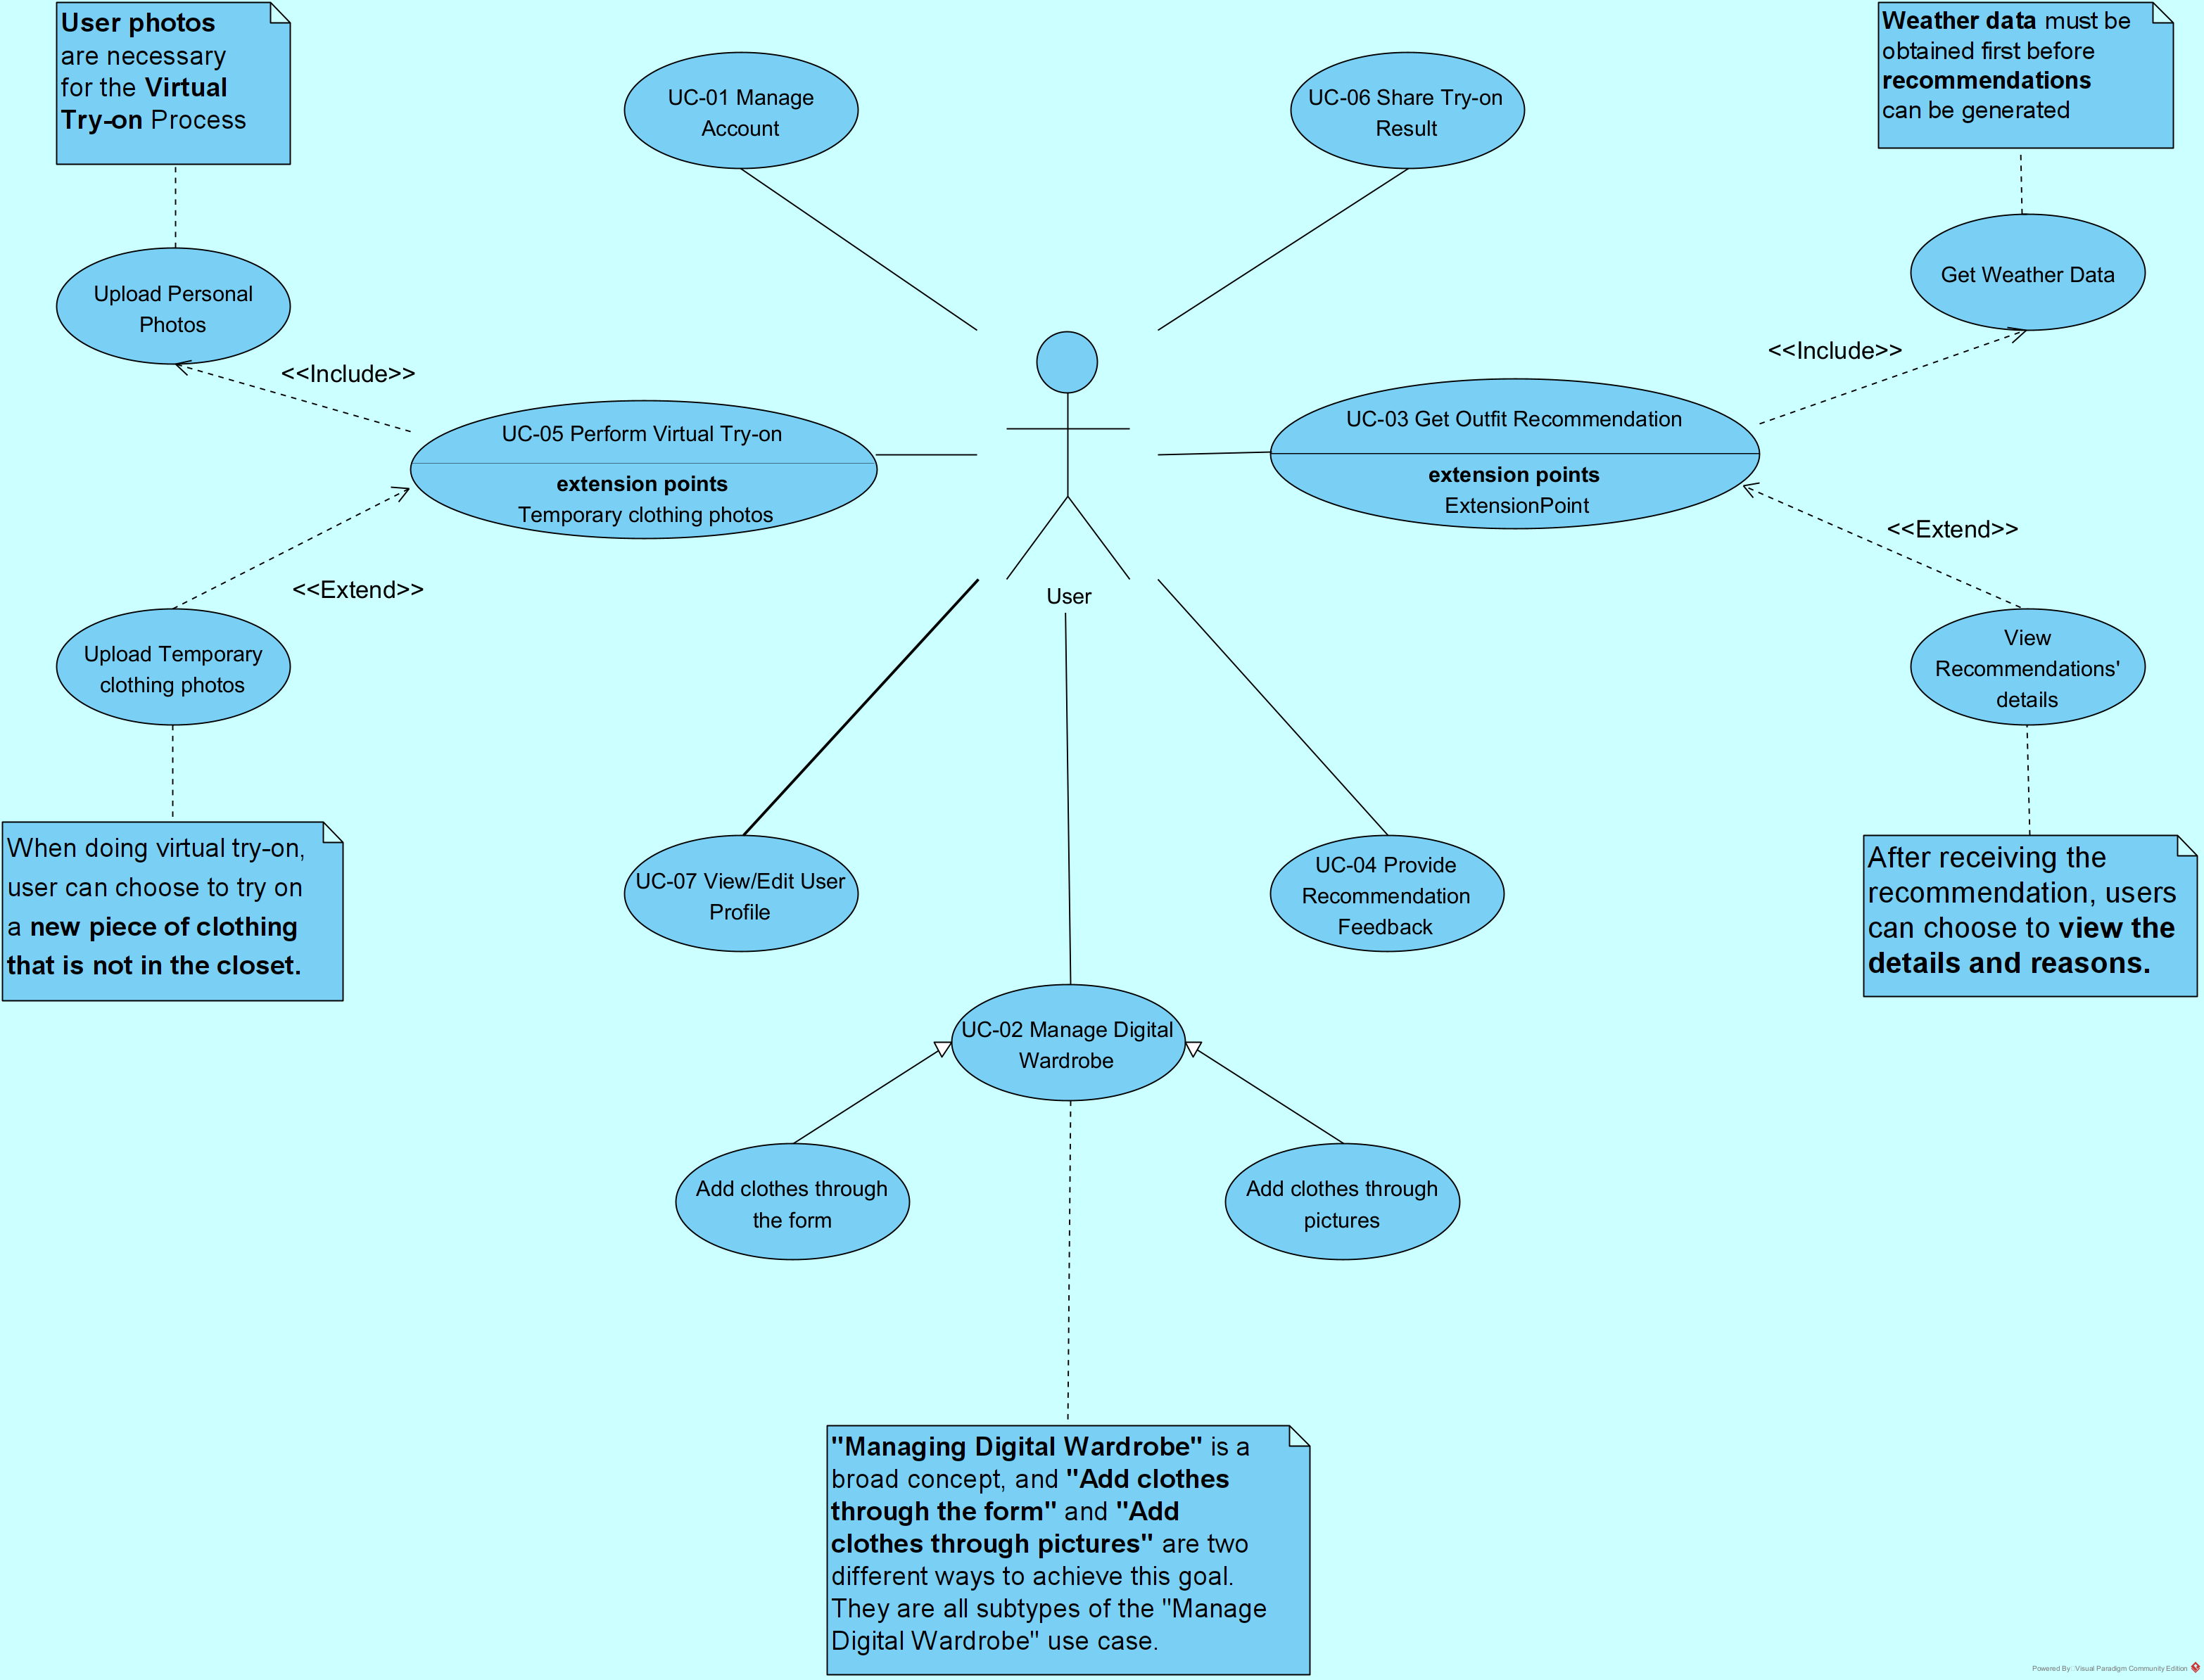
\includegraphics[width=1.0\textwidth]{images/Section_4_requirement/UCD.png}
    \caption{Use Case Diagram}
    \label{fig:UCD}
\end{figure}

Figure~\ref{fig:UCD} presents the overall use case diagram of the system.
Table~\ref{tab:uc_overview} below lists each use case in the diagram and briefly describes its functionality.

\begin{table}[H]
\centering
\caption{Use Case Overview}
\label{tab:uc_overview}
\begin{tabular}{p{4cm} p{12cm}}
\toprule
\textbf{Use Case ID} & \textbf{Brief Description} \\
\midrule
UC-01 Manage Account &
Users register, log in, or log out of the system. First-time users may complete initial wardrobe setup. \\
UC-02 Manage Digital Wardrobe &
Users add, edit, delete, and browse clothing items using forms or image uploads. The system processes and stores wardrobe entries. \\
UC-03 Get Outfit Recommendation &
The system generates personalized outfits based on preferences, weather, occasions, wardrobe items, and constraints, including explanations and alternatives. \\
UC-04 Provide Recommendation Feedback &
Users give feedback on recommendations (like/dislike/collect/not interested). The system updates preference models. \\
UC-05 Virtual Try-on &
Users upload photos or use wardrobe items to generate virtual try-on previews through body segmentation and overlay. \\
UC-06 Share Try-on Result &
Users export images or generate shareable links of their virtual try-on results. \\
UC-07 View/Edit User Profile &
Users view and edit preference profiles generated from wardrobe and interaction history. \\
\bottomrule
\end{tabular}
\end{table}



To ensure that the requirements are not merely conceptual but operationalized in actual workflows, each use case is explicitly linked to one or more functional requirements.

The following traceability matrix serves as a validation mechanism. It provides bi-directional traceability, confirming that no requirement is left unsupported and no use case is functionally unjustified.

\begin{table}[H]
\centering
\caption{Functional Requirements -- Use Case Traceability Matrix}
\label{tab:fr_uc_matrix}
\small
\setlength{\tabcolsep}{3pt}
\begin{tabular}{p{4cm} | c c c c c c c}
\toprule
\textbf{Functional Requirement} &
\textbf{UC-01} &
\textbf{UC-02} &
\textbf{UC-03} &
\textbf{UC-04} &
\textbf{UC-05} &
\textbf{UC-06} &
\textbf{UC-07} \\
\midrule
FR-01 Account registration/login                 & X &   &   &   &   &   &   \\
FR-02 Wardrobe creation (Form)                   &   & X &   &   &   &   &   \\
FR-03 Wardrobe creation (Image)                  &   & X &   &   &   &   &   \\
FR-04 User preferences (profile)                 &   &   & X & X &   &   & X \\
FR-05 Occasion and constraint input              &   &   & X &   &   &   &   \\
FR-06 Weather data acquisition                   &   &   & X &   &   &   &   \\
FR-07 Outfit recommendation                      &   &   & X &   &   &   &   \\
FR-08 Explanation / alternatives                 &   &   & X &   &   &   &   \\
FR-09 Feedback loop \& learning                  &   &   &   & X &   &   &   \\
FR-10 Virtual try-on (user photo)                &   &   &   &   & X &   &   \\
FR-11 Virtual try-on (clothing image)            &   &   &   &   & X &   &   \\
FR-12 Share try-on results                       &   &   &   &   &   & X &   \\
FR-13 Wardrobe maintenance                       &   & X &   &   &   &   &   \\
\bottomrule
\end{tabular}
\end{table}




\section{Requirement Validation}
\begin{itemize}
    \item \textbf{Traceability Validation}\\
As shown in the Functional Requirements--Use Case Traceability Matrix
(Table~\ref{tab:fr_uc_matrix}), every functional requirement is linked to at least
one use case, and no use case exists without originating from a defined
requirement. This ensures bidirectional traceability: (i) each requirement is
implemented through at least one user workflow, and (ii) each workflow has a
clear requirement basis defined in the SRS. This validation step helps prevent
missing functionality and unjustified features.

    \item \textbf{Supervisor Review and Confirmation}\\
    The core modules of the system --- wardrobe management, wardrobe analysis, outfit recommendation, and virtual try-on --- have been reviewed with the project supervisor and confirmed as the primary development priorities. During this review, the supervisor also verified that the main non-functional requirements are realistic and feasible under the current technical constraints.
    
\end{itemize}